\documentclass{report}

\usepackage[utf8]{inputenc}
\usepackage[french]{babel}
\usepackage{geometry}
\usepackage{helvet}
\usepackage{verbatim}
\usepackage{graphicx}
\usepackage{pdfpages}
\usepackage{caption} 

\title{Rapport du Projet de C++}
\author{LEMAN Jean-Christophe, CARON Alexandre, COLLOT Kévin}
\date{\today}

\pagestyle{headings}

\begin{document}
\maketitle
\tableofcontents


\chapter{Introduction}
\section{Présentation du sujet}
Le but de ce projet est de proposer une solution au problème du voyageur de commerce en utilisant un algorithme génétique.
\par Les algorithmes génétiques appartiennent à la famille des algorithmes évolutionnistes et sont basés sur les mécanismes et concepts du vivant comme par exemple les gènes, les chromosomes, la sélection naturelle ou encore les mutations génétiques. Ils permettent d'obtenir des solutions approchées à un problème d'optimisation là ou les méthodes mathématiques ne sont pas suffisamment efficaces.\par 
Le problème du voyageur de commerce en informatique est un problème d'optimisation, dans lequel étant donné un nombre de villes, ainsi que les distances séparant toutes les paires de villes, doit trouver un chemin le plus cours possible passant une et une seule fois par chacune des villes et terminant dans la ville de départ.
\section{Présentation du groupe}
Le trinôme est composé de:
\begin{itemize}
\item CARON Alexandre: chose
\item COLLOT Kévin: chose
\item LEMAN Jean-Christophe: chose
\end{itemize}

\chapter{Application}
\section{Spécifications de l'application}
\subsection{Présentation de l'application}
L'application est décomposée en de nombreuses classes ayant chacune un rôle précis et particulier. On retrouve des classes génériques, propres à tout algorithme génétique, ainsi que des classes spécifiques au problème du voyageur de commerce.\par 
L'aspect graphique de l'application est réalisé grâce à la bibliothèque CNG fournie par M.NGUYEN.
\subsection{Diagramme des cas d'utilisation}
	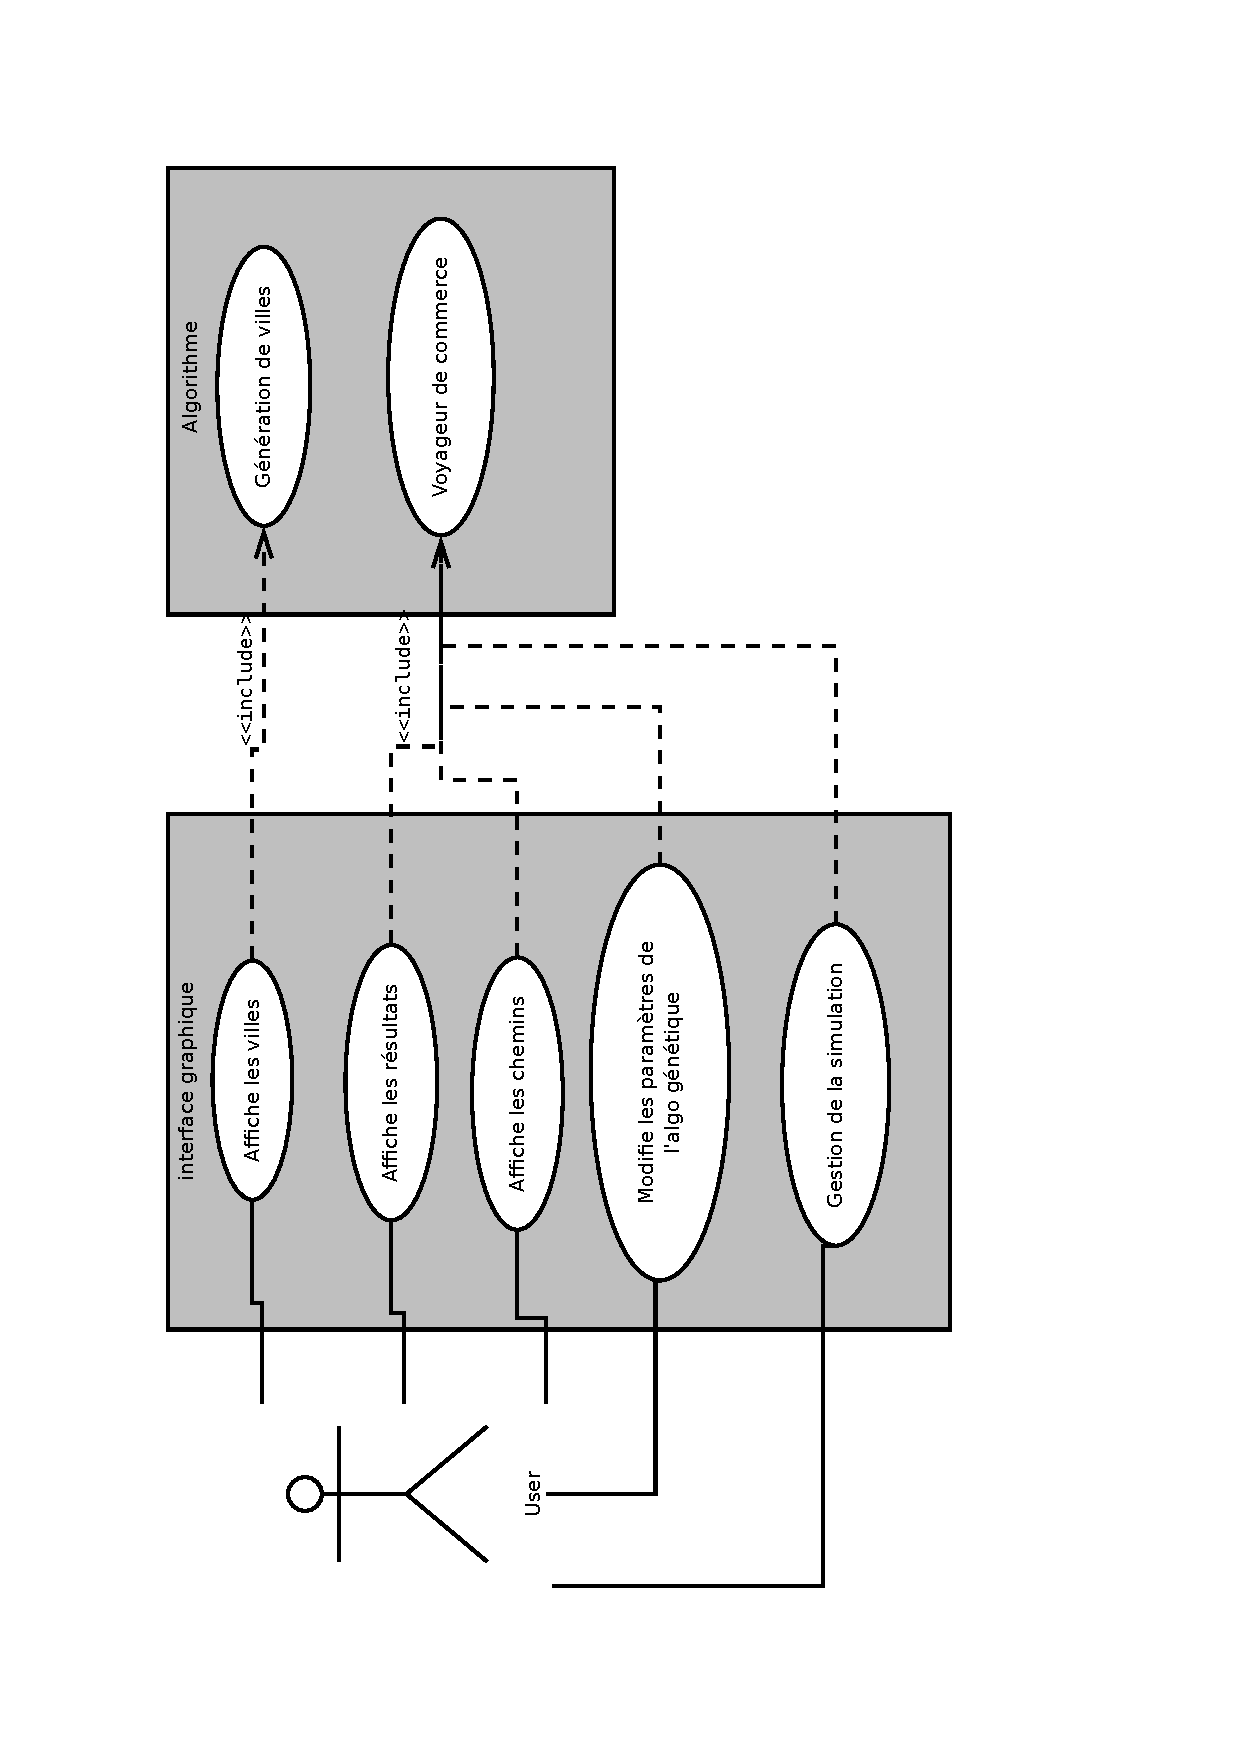
\includegraphics[scale=0.6, angle=270]{../UseCase.pdf}

\subsection{Diagramme des classes}
	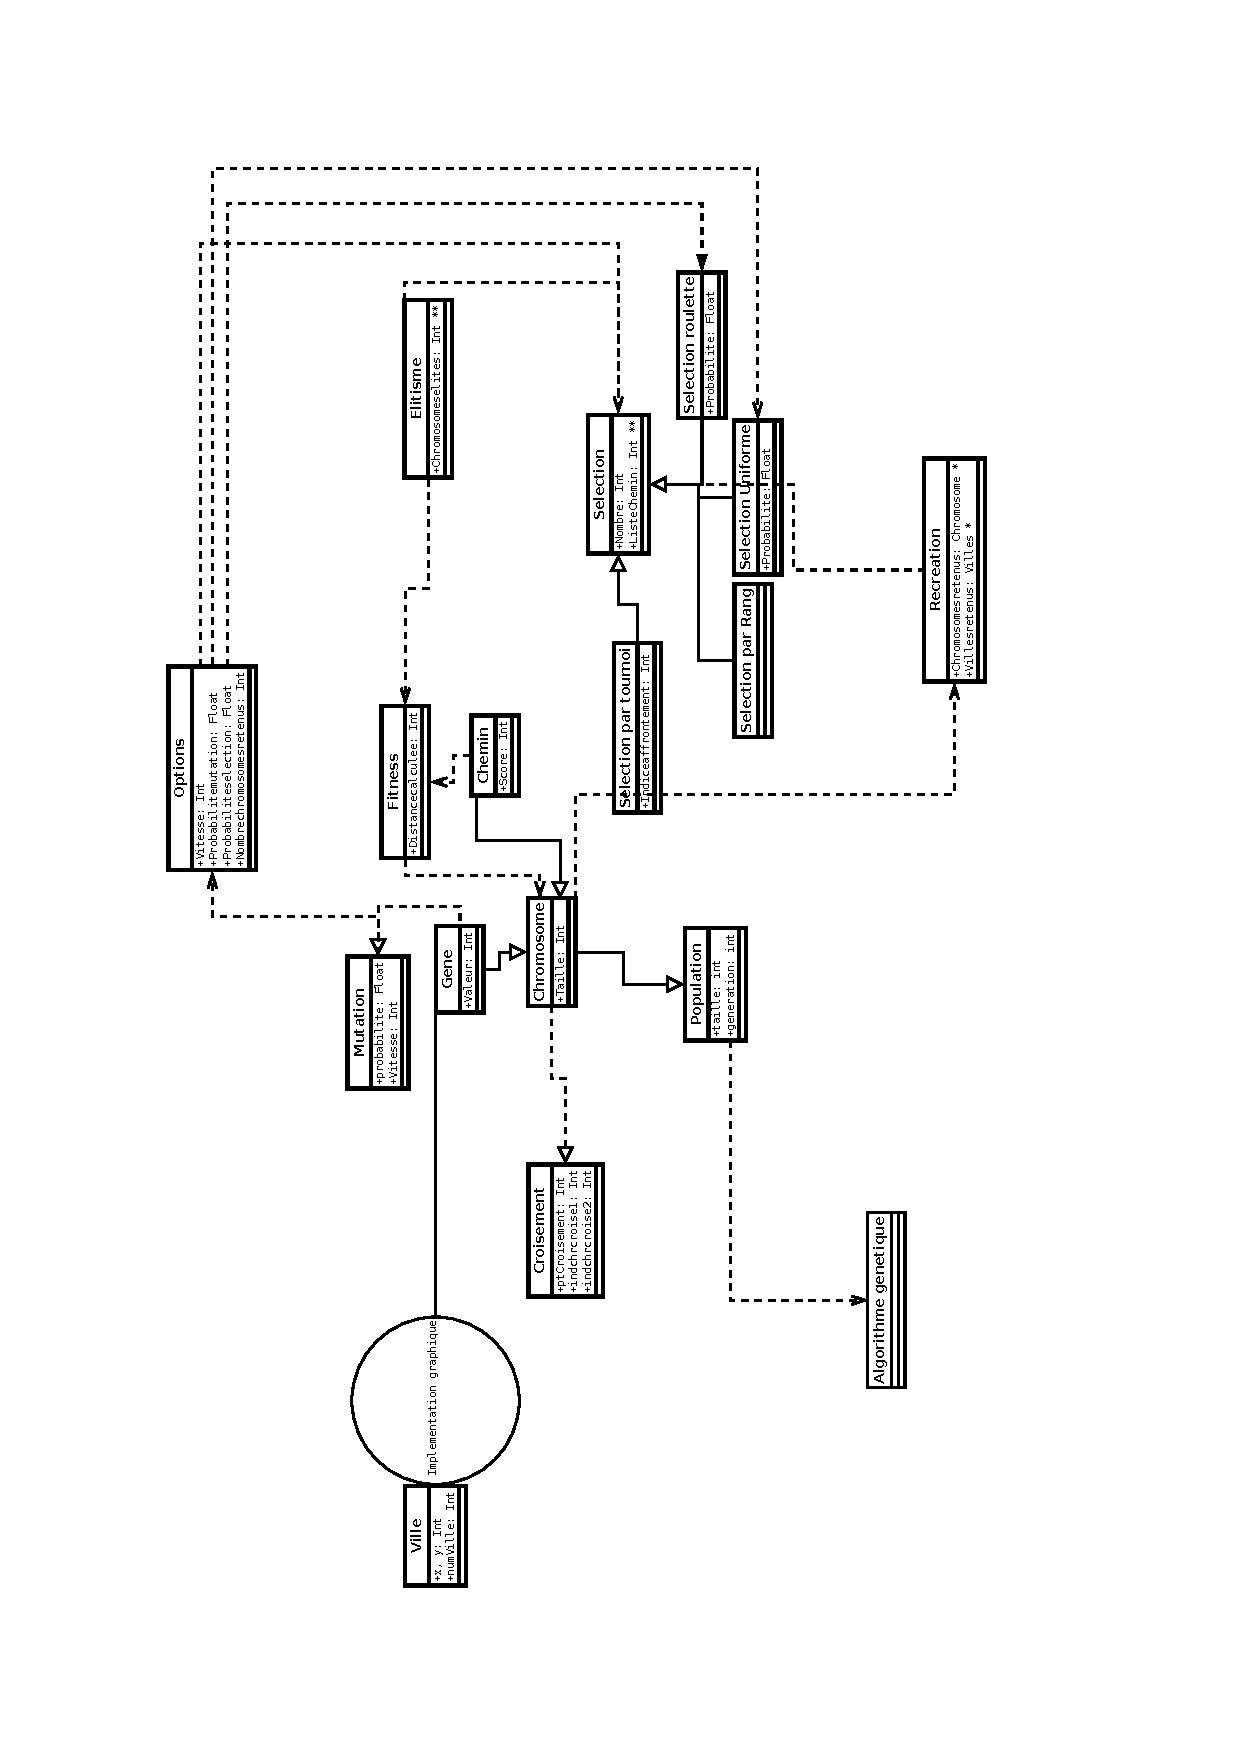
\includegraphics[scale=0.6, angle=270]{../Classes_UML.pdf}
\section{Manuel utilisateur}
Utiliser le makefile avec la commande make, puis lancer main.exe.
\chapter{Bilan}
\section{Difficultés rencontrées}
La notion d'algorithme génétique étant nouvelle, la première difficulté a été de saisir tous les aspects de ce type d'algorithme. Par la suite, le fait d'avoir à travailler sur de nombreuses classes a été une contrainte difficile à mettre en place, notamment pour dissocier convenablement les classes "génériques" des algorithmes génétiques des classes propres au problème du voyageur de commerce.
\section{Résultats obtenus}
\subsection{Capture d'écran d'une première génération}
	\begin{center}
		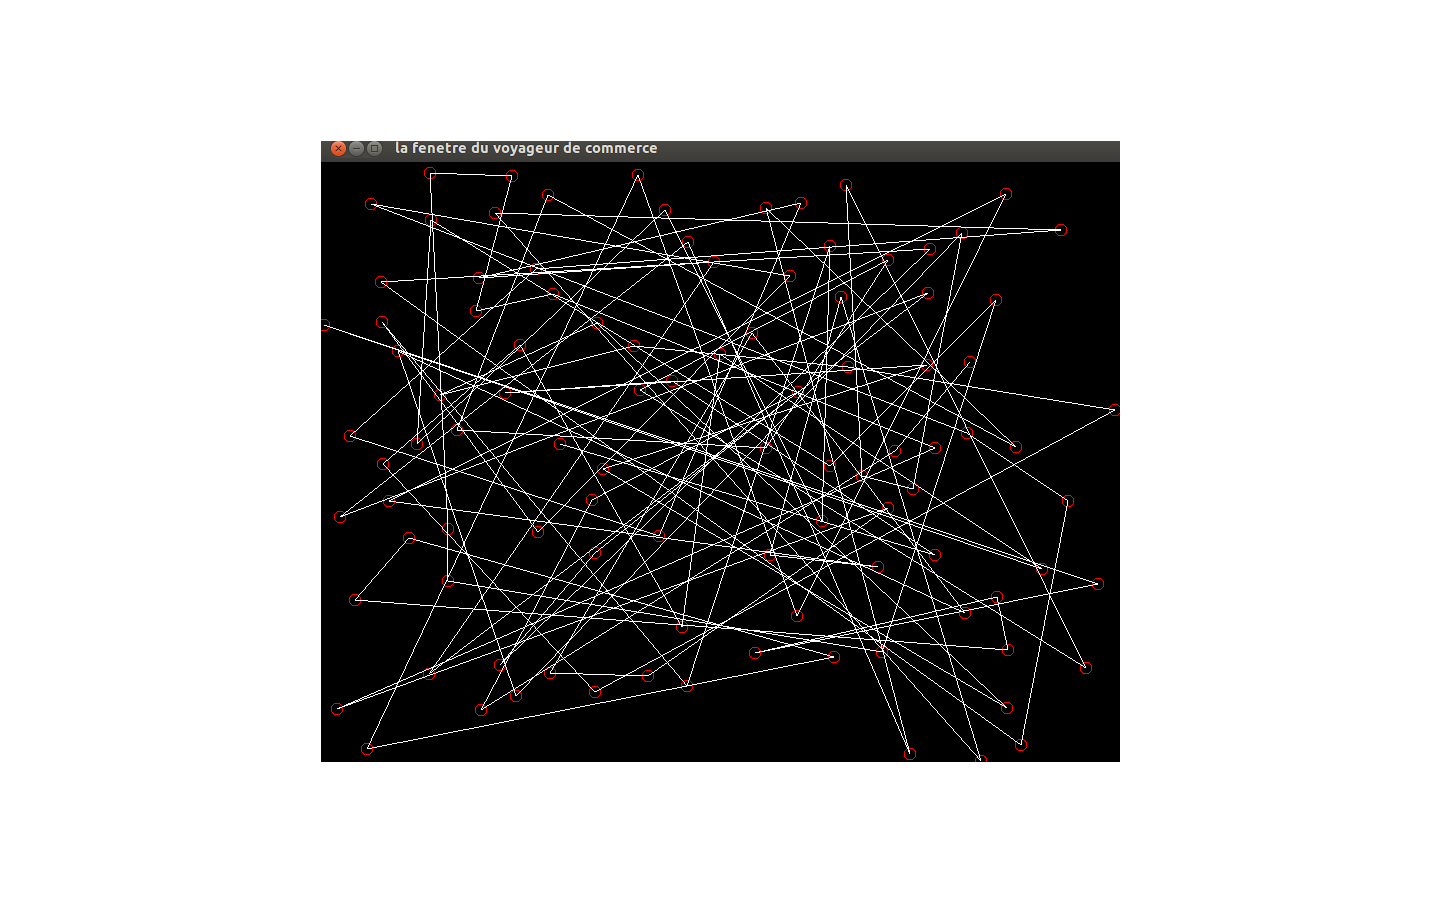
\includegraphics[scale=0.3]{./1erGeneration.png}
		\captionof{figure}{1ere génération.}
		\label{fig1}
	\end{center}
\section{Perspectives d'évolution}
On peut faire mieux.. On peut toujours faire mieux.


\end{document}